\documentclass[12pt,a4paper]{article}
\usepackage[UTF8]{ctex}
\usepackage{amsmath,amssymb}
\usepackage{xcolor}
\usepackage{hyperref}
\usepackage{geometry}
\usepackage{graphicx}
\geometry{margin=2.5cm}

\title{Fault-Tolerant Gate / 容错门}
\author{QuoNic}
\date{}

\begin{document}
\maketitle

\begin{center}
\textbf{Error Correction / 纠错} | 难度：高级 | 预计时间：20 分钟
\end{center}

\tableofcontents
\newpage

\section{为什么需要？}

容错门是在量子纠错码上执行的逻辑门。

\subsection{经典局限}
\begin{itemize}
  \item 普通量子门会传播错误
  \item 需要容错门避免错误传播
\end{itemize}

\subsection{量子优势}
\begin{itemize}
  \item 容错门可以避免错误传播
  \item 是容错量子计算的基础
  \item 提高量子计算的可靠性
\end{itemize}

\subsection{实际应用}
\begin{itemize}
  \item 容错量子计算
  \item 量子纠错
  \item 量子通信
\end{itemize}

\section{快速上手}

\begin{verbatim}
from quonic.qec import ft_gate

# 容错门
result = ft_gate(gate='H', code='steane')
print(f'Fault-tolerant circuit: {result.circuit}')
\end{verbatim}

\textbf{预期输出}：
\begin{verbatim}
Fault-tolerant circuit: ...
\end{verbatim}

\section{原理详解}

\subsection{电路图}

\begin{center}
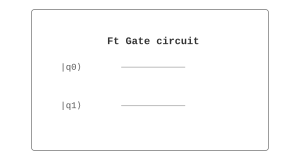
\includegraphics[width=0.6\textwidth]{../../images/ft_gate_circuit.svg}
\end{center}

\subsection{数学推导}

容错门：
\begin{equation}
U_L = \text{transversal}(U)
\end{equation}

其中 $U$ 是逻辑门，$U_L$ 是容错门。

\subsection{几何解释}

容错门在逻辑量子比特上执行操作，同时避免错误传播。

\section{代码详解}

\begin{verbatim}
from quonic.qec import ft_gate

# ft_gate(gate, code)
# gate: 逻辑门
# code: 纠错码

result = ft_gate(
    gate='H',
    code='steane'
)

# result.circuit: 容错电路
# result.depth: 电路深度
# result.gate_count: 门数量
print(f'Fault-tolerant circuit: {result.circuit}')
\end{verbatim}

\section{进阶用法}

\subsection{场景 1：不同纠错码}

\begin{verbatim}
from quonic.qec import ft_gate

# 不同纠错码
r1 = ft_gate(gate='H', code='steane')
r2 = ft_gate(gate='H', code='surface')
r3 = ft_gate(gate='H', code='color')
\end{verbatim}

\section{适用场景}

\subsection{容错量子计算}

容错门是容错量子计算的基础。容错门可以避免错误传播，提高量子计算的可靠性。

\subsection{量子纠错}

容错门用于量子纠错码上的逻辑操作。例如，在 Steane 码上执行 Hadamard 门。

\section{常见问题}

\subsection{容错门和普通门有什么区别？}

容错门可以避免错误传播，普通门会传播错误。

\subsection{容错门有哪些类型？}

常见的容错门包括：横向门、魔术态蒸馏门等。

\section{学习路径}

\subsection{前置知识}
\begin{itemize}
  \item 量子纠错码
  \item 量子门
  \item 量子测量
\end{itemize}

\subsection{继续学习}
\begin{itemize}
  \item 容错量子计算
  \item 魔术态蒸馏
  \item 量子硬件
\end{itemize}

\section{完整示例代码}

\subsection{示例 1：基本容错门}

\begin{verbatim}
from quonic.qec import ft_gate

result = ft_gate(gate='H', code='steane')
print(f'Fault-tolerant circuit: {result.circuit}')
\end{verbatim}

\section{下载}

\begin{itemize}
  \item [ft\_gate.py](https://github.com/ChrisLee0721/QuoNic/blob/main/examples/ft_gate/ft_gate.py)
\end{itemize}

\end{document}
